
\فصل{روش پیشنهادی}

فصل حاضر به شرح مراحل عملیاتی پروژه اختصاص دارد.
در این بخش ابتدا نحوه‌ی آماده‌سازی مجموعه‌داده شرح داده‌می‌شود.
سپس بررسی می‌شود که این تصاویر دستخوش چه تغییراتی شده و چگونه به مدل ورودی‌می‌شوند.
در انتها، طراحی انجام‌شده برای مدل یادگیری ماشین نیز توصیف خواهد شد.

\قسمت{آماده‌سازی مجموعه‌داده}

داده‌هایی که از مراکز پزشکی دریافت می‌شوند، مسیر طولانی‌ای را طی می‌کنند تا برای آموزش مدل قابل استفاده باشند.
اولین مرحله‌ی این آماده‌سازی شامل نگاشت اطلاعات بیماران به تصاویر می‌باشد.
این نگاشت از طریق شماره‌ی شناسه‌ی بیمار صورت می‌گیرد 
و در نتیجه‌ی آن، اطلاعات پزشکی در دسترس از بیماران به همراه مسیر ذخیره‌سازی تصاویر وی به صورت ساخت‌یافته‌ای جمع‌آوری می‌شوند.\
در پروژه‌ی حاضر نیز تصاویر CT مغزی از یک مرکز درمانی جمع‌آوری شده و مورد پژوهش قرار گرفته‌اند.

مرحله‌ی بعد، جداسازی تصاویر مورد توجه پژوهش است.
تصویربرداری‌های انجام‌شده از بیماران، معمولاً تنها شامل مغز نمی‌شوند و تصاویری از ریه و \dots را نیز در بر دارند.
به علاوه در هر مجموعه، تعداد تصاویر مغزی نیز با مجموعه‌های دیگر می‌تواند تفاوت داشته باشد.
به گونه‌ای که یک بیمار ۱۵ و بیمار دیگر، ۵۰ برش از مغز را در مجموعه‌ی خود داشته باشد.
این در حالی است که در امتیازدهی ASPECTS تنها چند برش خاص از مغز مورد استفاده قرار می‌گیرد.
به این ترتیب، یکی از گام‌های ضروری برای آماده‌سازی داده‌ها، جداسازی این برش‌ها از میان تمام 
تصاویر دریافت‌شده از بیماران و تهیه‌ی یک نگاشت مدون از هر بیمار به برش‌های استخراج‌شده از تصاویر وی می‌باشد.

با انجام دو اقدام فوق که بیشتر مربوط به مرتب‌سازی و خالص‌سازی اطلاعات بودند، نوبت به مرحله‌ی 
پیش‌پردازش\footnote{Pre-processing}
تصاویر می‌رسد.
پیش‌پردازش یکی از مهم‌ترین و موثرترین گام‌های یادگیری ماشین محسوب می‌شود که ارتباط مستقیمی با عملکرد و توانایی یادگیری مدل دارد. 
درواقع پیش‌پردازش شامل تغییراتی در داده‌های ورودی است که باعث می‌شود تا جای ممکن، اطلاعات نامفید از داد‌ه‌ها حذف شوند و اطلاعات کلیدی نیز در قالب مناسبی به مدل عرضه شوند.
به این ترتیب فرایند یادگیری برای مدل ساده‌تر خواهد بود.

نکته‌ی دیگری که باعث اهمیت بیشتر پیش‌پردازش می‌شود، قابلیت استفاده‌ی مجدد آن در پژوهش‌های دیگر است.
درواقع گام‌های پیش‌پردازش تصاویر پزشکی در بسیاری از پژوهش‌ها با هم اشتراکات زیادی دارد.
روش‌های ارائه شده در این پروژه نیز می‌توانند در پیش‌پردازش تصاویر CT در سایر تحقیقات راهگشا باشند.
در ادامه، فرایند پیش‌پردازش مورد استفاده در این پژوهش، به صورت گام به گام بر روی یک تصویر مغزی انتخابی شرح داده می‌شوند.\footnote{در طراحی مراحل پیش‌پردازش این پروژه، مرجع \cite{ma2020medical} به‌کار آمده‌است.}

\زیرقسمت{افزایش وضوح}
همانطور که در بخش مفاهیم اولیه ذکر شد، مقدار عددی هر پیکسل در تصاویر پزشکی، بازه‌ی بزرگی را شامل می‌شود.
این در حالی است که چشم انسان تنها تعداد محدودی رنگ خاکستری را می‌تواند از هم تمیز دهد.
به همین دلیل، در صورت مشاهده‌ی یک تصویر CT خام، جزئیات بافت مغز و حتی ناحیه‌ی آسیب‌دیده، قابل مشاهده نخواهد بود. 
با این توضیح، تصویر انتخابی برای شرح مراحل پیش‌پردازش، در ابتدا مانند 
شکل \ref{fig:raw-ct} است.\footnote{ناحیه‌ی مغز برای مقاصد نمایشی، کمی جا‌به‌جا شده‌است.}
بنابراین، در اولین گام، لازم است وضوح تصاویر افزایش داده‌شود.

% \begin{figure}[ht]
% \centering
% 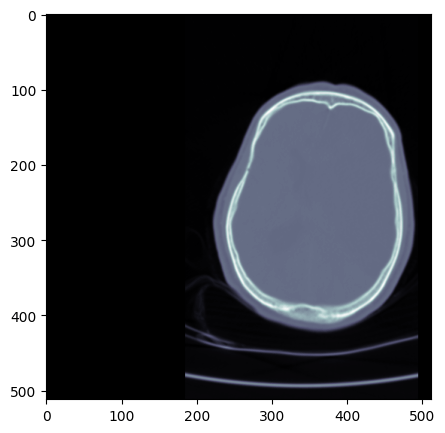
\includegraphics[width=\textwidth, keepaspectratio]{raw-ct.png}
% \caption[]{تصویر انتخابی برای نمایش مراحل پیش‌پردازش، در حالت اولیه.}
% \label{fig:raw-ct}
% \end{figure}

\شروع{شکل}[ht]
\centerimg{raw-ct}{0.5\textwidth}
\شرح[تصویر نمونه پیش‌پردازش]{تصویر انتخابی برای نمایش مراحل پیش‌پردازش، در حالت اولیه.}
\برچسب{fig:raw-ct}
\پایان{شکل}

 میان مقدار هر پیکسل با بافت یا شیئی که نمایش می‌دهد ارتباط وجود دارد.
به نحوی که آب، مقدار $0 HU$، هوا مقدار $-1000 HU$، بافت استخوانی مقدار $1000 HU$ و بافت مغزی در حدود $20-50 HU$ می‌باشد \cite{kamalian2016computed}.
به این ترتیب، با محدود کردن مقدار پیکسل‌ها به بازه‌ای مثل $0-100 HU$، اطلاعات مربوط به بافت مغز از بین نمی‌رود.
اما این بار به علت کاهش بازه‌ی رنگ خاکستری، اجزای تصویر از هم بهتر تمایز می‌یابند.
در اصطلاح تصاویر پزشکی، به بازه‌ای که مقادیر به آن محدود می‌شوند 
پهنای پنجره\footnote{\lr{Window Width}}
و به مرکز این بازه
 سطح پنجره\footnote{\lr{Window Level}} گفته می‌شود.
با اعمال پهنای پنجره‌ی 100 و سطح پنجره‌ی ۵۰، تصویر اولیه مانند شکل 
\ref{fig:windowed-ct}
می‌شود.

% \begin{figure}[ht]
% \centering
% 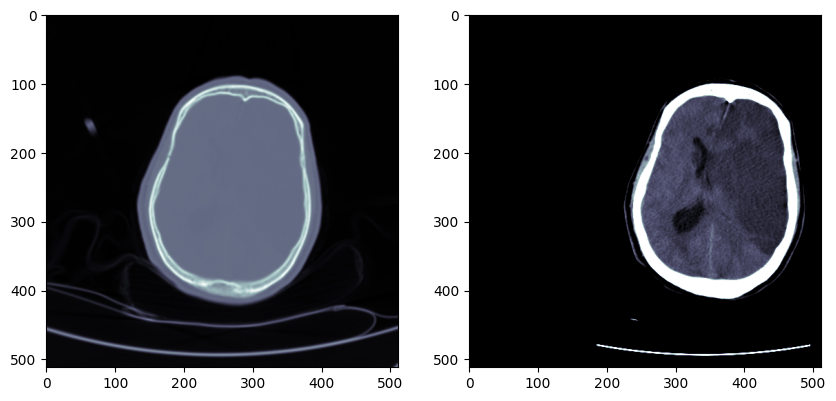
\includegraphics[width=\textwidth, keepaspectratio]{windowed-ct.png}
% \caption[]{تصویر انتخابی برای نمایش مراحل پیش‌پردازش، پیش و پس از تنظیم پهنای پنجره به 100 و سطح پنجره به ۵۰. سمت راست، تصویر پس از تنظیم پنجره را نمایش می‌دهد.}
% \label{fig:windowed-ct}
% \end{figure}

\شروع{شکل}[ht]
\centerimg{windowed-ct}{0.8\textwidth}
\شرح[تنظیم پهنا و سطح پنجره‌ی تصاویر ]{تصویر انتخابی برای نمایش مراحل پیش‌پردازش، پیش و پس از تنظیم پهنای پنجره به 100 و سطح پنجره به ۵۰. سمت راست، تصویر پس از تنظیم پنجره را نمایش می‌دهد.}
\برچسب{fig:windowed-ct}
\پایان{شکل}


روش معمول برای افزایش وضوح تصاویر، به همین صورت با تنظیم پهنا و سطح پنجره می‌باشد.
اما باید توجه داشت که میان تصاویر بیماران مختلف، تفاوت‌های جزئی وجود دارد.
برخی تصاویر ممکن است به طور کلی قدری تیره‌تر و یا روشن‌تر باشند.
در نتیجه اعمال یک سیاست واحد برای پهنا و سطح پنجره ممکن است برای تمام تصاویر، بهینه نباشد و وضوح لازم را برای تصویر فراهم نکند.
در این پژوهش، از یک روش پویا برای تنظیم وضوح تصاویر استفاده شده‌است که شرح آن در ادامه می‌آید.

در این روش، ابتدا مقدار پیکسل‌های مربوط به بافت مغزی هر بیمار به صورت یک مجموعه، استخراج می‌شوند.
سپس چند درصد پایین و چند درصد بالای این مقادیر محاسبه می‌شوند.
در نتیجه، یک 
چندک\footnote{Quantile} 
پایین و یک چندک بالا به‌دست می‌آید.
در نهایت، مقادیر پیکسل‌های کل تصویر، محدود به بازه‌ی میان این دو چندک می‌شوند.
به این ترتیب، در هر تصویری، با توجه به اطلاعات آماری همان تصویر، 
مقدار پیکسل‌ها محدود به بازه‌ای از رنگ خاکستری می‌شود که اطلاعات بیشتری در خود دارد.
اعمال این روش پویا، نیازمند استخراج بافت مغزی است که در مراحل انتهایی پیش‌پردازش به‌دست می‌آید.
به همین جهت، از آوردن تصویر آن در این بخش صرف نظر می‌شود
اما تصویر نهایی فرایند پیش‌پردازش، نمایانگر افزایش بیشتر وضوح 
تصاویر نسبت به روش‌های ایستا (مانند تصویر \ref{fig:windowed-ct}) می‌باشد.

\زیرقسمت{کاهش نویز}

تصاویر اخذ شده از بیماران معمولاً دارای نویز هستند.
گاهی این نویز بسیار شدید است و گاهی جزئی بوده و تشخیص آن در نگاه کلی مشکل است.
در این پژوهش، تصاویری که دارای نویز شدید بودند، از مجموعه‌داده حذف شده‌اند.
اما در مورد سایر تصاویر، همچنان نویز اندکی باقی می‌ماند.
در فرایند پیش‌پردازش پیشنهادی، این نویز با دو مرتبه اعمال 
فیلتر میانه\footnote{\lr{Median Filtering}}
در تصاویر، کاهش می‌یابد.

فیلتر میانه به این صورت عمل می‌کند که مقدار هر پیکسل را 
با میانه‌ی پیکسل‌های مجاورش در یک همسایگی مشخص جایگزین می‌کند.
به این ترتیب، اگر تعداد اندکی پیکسل در آن همسایگی، مقادیر پرتی داشته باشند، با مقادیری در محدوده‌ی مناسب، ترمیم می‌شوند.
شدت کاهش نویز به اندازه‌ی همسایگی مورد بررسی در فیلتر میانه بستگی دارد.
هر چه این پنجره بزرگ‌تر باشد، تصویر خروجی محو‌تر و در هم تنیده‌تر
می‌شود.
در مقابل، هر چه فیلتر کوچک‌تر باشد، توانایی کاهش نویزش هم به جمعیت کوچک‌تری محدود می‌شود و برای رفع نویز‌های سنگین مناسب نخواهد بود.

همانطور که پیش‌تر ذکر شد، در پیش‌پردازش پیشنهادی در این پژوهش، فیلتر میانه دو مرتبه اعمال می‌شود. 
یک مرتبه با پنجره‌ای با اندازه‌ی $7 \times 7$ پیکسل و یک مرتبه با اندازه‌ی $3 \times 3$ پیکسل.
این مقادیر با آزمون و خطا بر روی تصاویر به‌دست آمده‌اند و علاوه بر کاهش نویز، باعث محو شدن و حذف جزئیات غیر مهم در عکس می‌شوند.
این محو‌سازی در افزایش وضوح تصویر نیز تاثیر به‌سزایی دارد.
چرا که در این صورت، مقادیر دورافتاده در میان پیکسل‌ها، حد بالا و پایین پنجره‌ی وضوح را محدود نمی‌کنند.
نمونه‌ی اعمال فیلتر به این روش بر روی تصویر انتخابی 
در شکل
\ref{fig:denoised-ct}
آمده‌است.

% \begin{figure}[ht]
% \centering
% 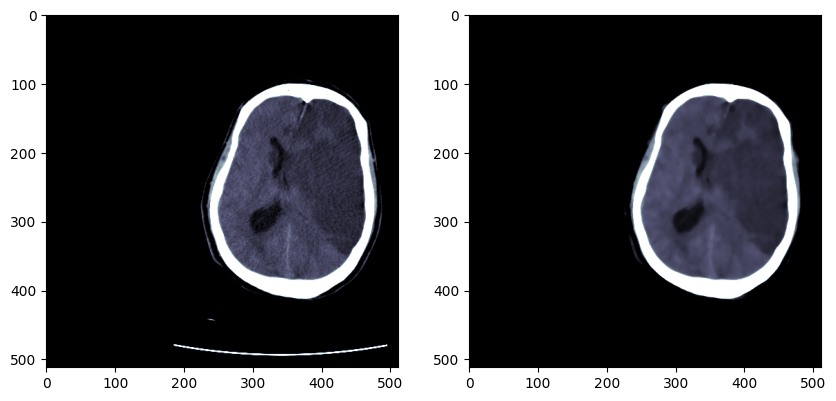
\includegraphics[width=\textwidth, keepaspectratio]{denoised-ct.png}
% \caption[]{تصویر انتخابی برای نمایش مراحل پیش‌پردازش، پیش و پس از اعمال فیلتر میانه. سمت راست تصویر پس از اعمال فیلتر را نشان می‌دهد.}
% \label{fig:denoised-ct}
% \end{figure}

\شروع{شکل}[ht]
\centerimg{denoised-ct}{0.8\textwidth}
\شرح[اعمال فیلتر میانه بر تصاویر]{تصویر انتخابی برای نمایش مراحل پیش‌پردازش، پیش و پس از اعمال فیلتر میانه. سمت راست تصویر پس از اعمال فیلتر را نشان می‌دهد.}
\برچسب{fig:denoised-ct}
\پایان{شکل}
    
\زیرقسمت{تنظیم زاویه}
تصاویر مغز ممکن است به دلایلی چون حرکت سر بیمار، همگی زاویه‌ی یکسانی نداشته‌باشند.
به منظور یک‌دست سازی تصاویر از این جهت، ابتدا ناحیه‌ی سر به صورت یک بیضی تخمین زده می‌شود و سپس با دوران حول یکی از قطر‌هایش، در زاویه‌ی قائم قرار می‌گیرد.
نمونه‌ی این محاسبات و تغییرات در تصویر انتخابی در شکل \ref{fig:aligned-ct}
قابل مشاهده است.

% \begin{figure}[ht]
% \centering
% 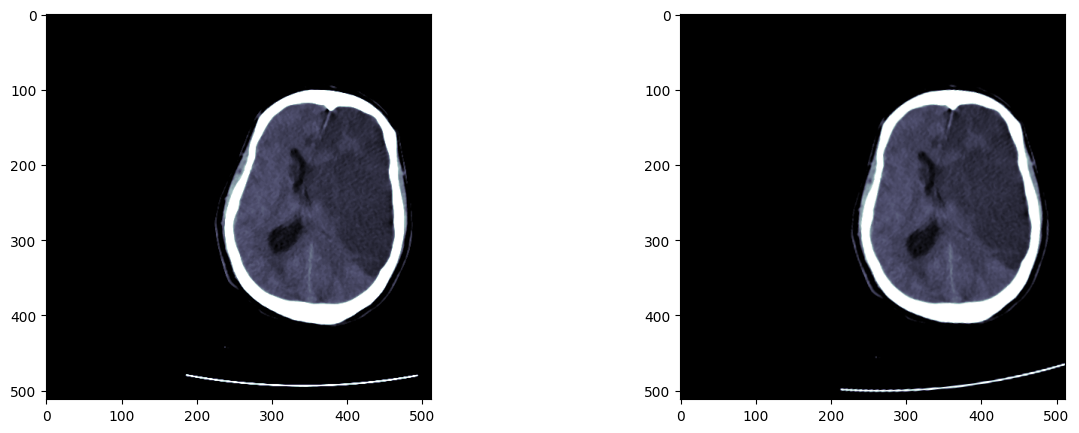
\includegraphics[width=\textwidth, keepaspectratio]{aligned-ct.png}
% \caption[]{تصویر انتخابی برای نمایش مراحل پیش‌پردازش، پیش و پس از تنظیم زاویه. سمت راست تصویر پس از تنظیم زاویه را نشان می‌دهد.}
% \label{fig:aligned-ct}
% \end{figure}

\شروع{شکل}[ht]
\centerimg{aligned-ct}{0.8\textwidth}
\شرح[تنظیم زاویه‌ی تصاویر]{تصویر انتخابی برای نمایش مراحل پیش‌پردازش، پیش و پس از تنظیم زاویه. سمت راست تصویر پس از تنظیم زاویه را نشان می‌دهد.}
\برچسب{fig:aligned-ct}
\پایان{شکل}

\زیرقسمت{محدودسازی تصویر به ناحیه‌ی مغز}
به دلایل مشابه قسمت قبل، ناحیه‌ی مغز بیمار ممکن است دقیقاً در مرکز تصویر قرار نداشته باشد.
علاوه بر این، چنانکه در تصویر \ref{fig:aligned-ct} مشخص است، 
در هر تصویر، هوای اطراف سر بیمار و گاهی حتی بخش‌هایی دستگاه تصویربرداری نیز حضور دارد.
مقدار این اضافات نیز از تصویری به تصویر دیگر متفاوت است.
یکی از مراحل پیش‌پردازش مربوط به همین مسئله می‌باشد.

در این مرحله،
با برش تصویر و محدودسازی آن به ناحیه‌ی مغز،
علاوه بر اینکه مغز بیمار در مرکز تصویر قرار می‌گیرد، اضافات موجود در تصویر از آن حذف می‌شود.
لازم به ذکر است از آن‌جا که ابعاد مغز بیماران متفاوت است، تصاویر حاصل از این مرحله، همگی به یک ابعاد جدید و مشخص، تغییر اندازه نیز می‌یابند.
خروجی این مرحله بر روی تصویر نمونه در شکل 
\ref{fig:resized-ct}
آمده‌است.

% \begin{figure}[ht]
% \centering
% 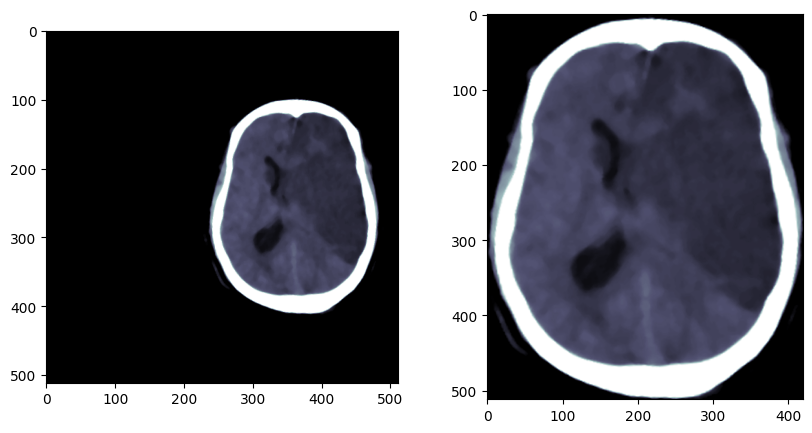
\includegraphics[width=\textwidth, keepaspectratio]{resized-ct.png}
% \caption[]{تصویر انتخابی برای نمایش مراحل پیش‌پردازش، پیش و پس از محدودسازی به ناحیه‌ی مغز. سمت راست، تصویر پس از محدودسازی و استانداردسازی ابعاد را نشان می‌دهد.}
% \label{fig:resized-ct}
% \end{figure}

\شروع{شکل}[ht]
\centerimg{resized-ct}{0.8\textwidth}
\شرح[تنظیم ابعاد تصاویر]{تصویر انتخابی برای نمایش مراحل پیش‌پردازش، پیش و پس از محدودسازی به ناحیه‌ی مغز. سمت راست، تصویر پس از محدودسازی و استانداردسازی ابعاد را نشان می‌دهد.}
\برچسب{fig:resized-ct}
\پایان{شکل}

\زیرقسمت{حذف استخوان جمجمه}

طبیعتاً تمام برش‌های مغز شامل بخشی از استخوان جمجمه در اطراف مغز هستند.
اما این بافت استخوانی، به هر صورت، اطلاعات زائد و فاقد اهمیت در تشخیص سکته‌ی مغزی محسوب می‌شود.
هر چه اطلاعات نامربوط کمتری به مدل عرضه شود، توانایی آن در یادگیری صحیح ویژگی‌های کلیدی نیز افزایش می‌یابد.
به همین منظور، مرحله‌ی بعدی پیش‌پردازش، به 
حذف استخوان جمجمه\footnote{\lr{Skull Stripping}}
و یا 
استخراج بافت مغز\footnote{\lr{Brain Extraction}}
از تصاویر اختصاص دارد.

روش‌های مختلفی برای این کار وجود دارد.
یک روش، آموزش یک مدل مجزا برای ناحیه‌بندی استخوان جمجمه می‌باشد.
روش دیگر، استفاده از انطباق تصاویر است که در بخش مفاهیم اولیه به آن اشاره شد.
به این معنا که هر تصویر جدید، با یک تصویر استاندارد با ناحیه‌بندی مشخص برای بافت مغز، انطباق داده شود و بافت مغزی متناظر با آن از تصویر جدید استخراج گردد.
اما روش اول زمان‌بر بوده و نیازمند تعداد زیادی تصویر با برچسب ناحیه‌ی استخوان جمجمه برای هر پیکسل است.
روش دوم نیز گاهی نادقیق عمل می‌کند.
در این پژوهش از روش اعمال آستانه بر روی مقدار پیکسل‌ها استفاده می‌شود که شرح آن در ادامه خواهد آمد.

در این روش، از این حقیقت استفاده می‌شود که بافت استخوانی، چنانکه در بخش افزایش وضوح آمد، دارای بیشترین مقدار در واحد HU است.
به این ترتیب با اعمال یک حد آستانه بر روی مقدار پیکسل‌ها، می‌‌توان این بافت را از تصویر حذف کرد.
البته در این رابطه چالش هایی نیز وجود دارد.
زیرا با حذف این مقادیر، یک‌سری پیکسل‌ها در میانه‌ی بافت مغز نیز حذف می‌شوند و حفره‌هایی در آن ایجاد می‌شود.
همچنین در برخی تصاویر، ممکن است بافت‌های نازکی در اطراف استخوان جمجمه وجود داشته باشند که با اعمال حد آستانه حذف نشوند.

به منظور رفع این مشکلات، پس از اعمال آستانه، از برخی روش‌های 
ریخت‌شناسی\footnote{Morphology}
در پردازش تصویر استفاده می‌شود تا
حفره‌های کوچک تصویر حاصل پر شوند و 
خطوط باریکی که به عنوان بافت مغز تشخیص داده‌شده‌اند، حذف گردند.
نمونه‌ی استخراج بافت مغزی به این روش بر روی تصویر نمونه، در شکل \ref{fig:skull-stripped-ct}
قابل مشاهده است.

% \begin{figure}[ht]
% \centering
% 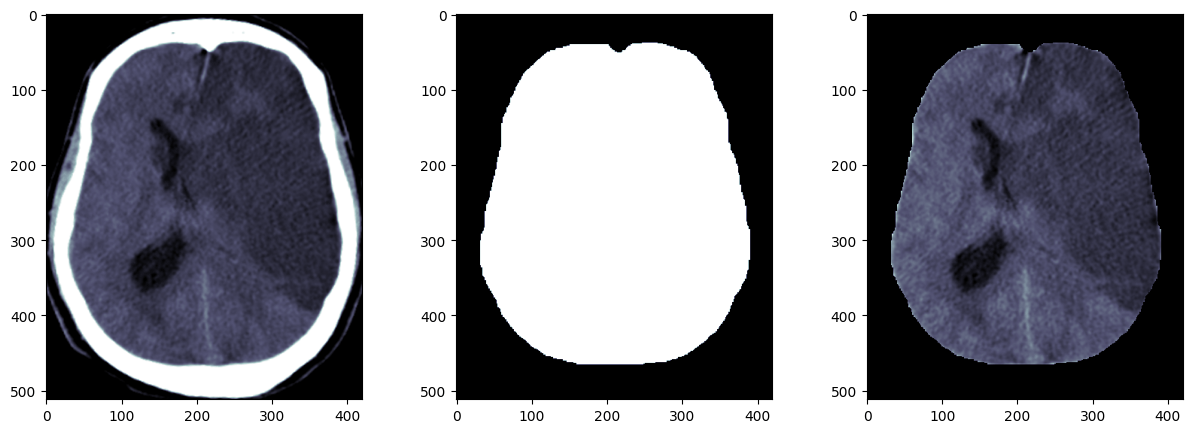
\includegraphics[width=\textwidth, keepaspectratio]{skull-stripped-ct.png}
% \caption[]{تصویر انتخابی برای نمایش مراحل پیش‌پردازش، پیش و پس از حذف استخوان جمجمه. تصویر وسط، ناحیه‌ی تشخیص داده‌شده به عنوان بافت مغز و سمت راست تصویر حاصل از حذف استخوان جمجمه را نشان می‌دهد.}
% \label{fig:skull-stripped-ct}
% \end{figure}

\شروع{شکل}[ht]
\centerimg{skull-stripped-ct}{\textwidth}
\شرح[حذف استخوان جمجمه از تصاویر]{تصویر انتخابی برای نمایش مراحل پیش‌پردازش، پیش و پس از حذف استخوان جمجمه. تصویر وسط، ناحیه‌ی تشخیص داده‌شده به عنوان بافت مغز و سمت راست تصویر حاصل از حذف استخوان جمجمه را نشان می‌دهد.}
\برچسب{fig:skull-stripped-ct}
\پایان{شکل}

همانطور که در قسمت افزایش وضوح ذکر شد پس از تکمیل این مرحله، ناحیه‌ی تشخیص داده‌شده به عنوان بافت مغز، برای تحلیل‌های آماری بر روی مقدار پیکسل‌های بافت مغز مورد استفاده قرار می‌گیرد و در افزایش وضوح تصویر به‌کار می‌آید.
با استفاده از این روش، وضوح تصاویر و تمایز بافت سالم از آسیب‌دیده، به طور قابل توجهی افزایش می‌یابد.
شکل \ref{fig:preprocessing-pipeline}
مراحل کامل پیش‌پردازش بر روی تصویر انتخابی و نتیجه‌ی نهایی آن را نشان می‌دهد.

% \begin{figure}[ht]
% \centering
% 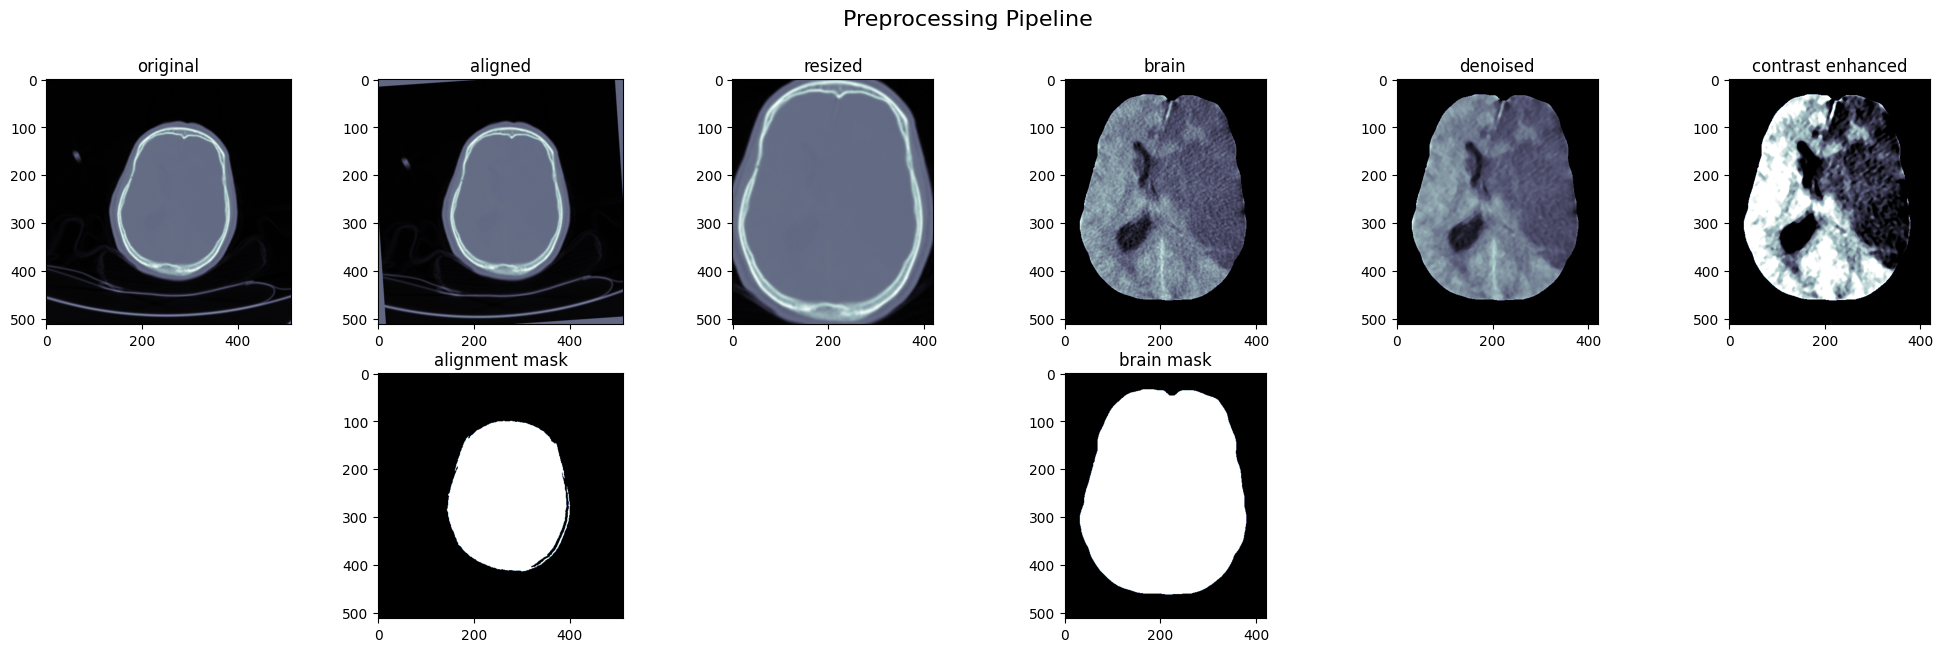
\includegraphics[width=\textwidth, keepaspectratio]{preprocessing-pipeline.png}
% \caption[]{مراحل کامل فرایند پیش‌پردازش بر روی تصویر انتخابی. از چپ به راست ، این مراحل شامل تنظیم زاویه، محدودسازی به ناحیه‌ی مغز، حذف استخوان جمجمه، کاهش نویز و افزایش وضوح می‌باشند. دو تصویر ردیف پایین نیز از چپ به راست، ناحیه‌ی تشخیص داده‌شده به عنوان سر (با تخمین سر به صورت بیضی) و ناحیه‌ی تشخیص داده‌شده به عنوان بافت مغز را نشان می‌دهند.}
% \label{fig:preprocessing-pipeline}
% \end{figure}

\شروع{شکل}[ht]
\centerimg{preprocessing-pipeline}{\textwidth}
\شرح[مراحل کامل پیش‌پردازش]{مراحل کامل فرایند پیش‌پردازش بر روی تصویر انتخابی. از چپ به راست ، این مراحل شامل تنظیم زاویه، محدودسازی به ناحیه‌ی مغز، حذف استخوان جمجمه، کاهش نویز و افزایش وضوح می‌باشند. دو تصویر ردیف پایین نیز از چپ به راست، ناحیه‌ی تشخیص داده‌شده به عنوان سر (با تخمین سر به صورت بیضی) و ناحیه‌ی تشخیص داده‌شده به عنوان بافت مغز را نشان می‌دهند.}
\برچسب{fig:preprocessing-pipeline}
\پایان{شکل}


\قسمت{داده‌افزایی}

زمانی که داده‌ها پیش‌پردازش شوند، آماده‌ی عرضه به مدل خواهند بود.
اما همانطور که پیش‌تر ذکر شد، تعداد این داده‌ها محدود است و مدل نمی‌تواند یادگیری قابل اعتمادی از این تعداد تصویر داشته‌باشد.
بنابراین
 با مقدمه‌ای که در فصل مفاهیم اولیه آمد، لازم است حجم تصاویر با روش‌های مناسبی افزایش یابد.
 این روش‌ها در قالب داده‌افزایی مطرح می‌شوند.
 در این قسمت به روش‌های داده‌افزایی مورد استفاده در این پژوهش اشاره می‌شود.

 اولین تکنیک داده‌افزایی مورد استفاده، قرینه‌سازی تصادفی تصویر مغز است.
 به این معنا که جای نیم‌کره‌ی چپ و راست هر تصویر ورودی، در هر بار مشاهده توسط مدل، به صورت تصادفی
 عوض می‌شود.
 به این ترتیب اگر یک تصویر با آسیب‌دیدگی در نیم‌کره‌ی چپ در مجموعه‌داده وجود داشته باشد، مدل می‌تواند آسیب‌دیدگی در نیم‌کره‌ی راست را نیز بیاموزد.
 یک نمونه از این داده‌افزایی در شکل \ref{fig:horizontal-flip} قابل مشاهده است.

%  \begin{figure}[ht]
% \centering
% 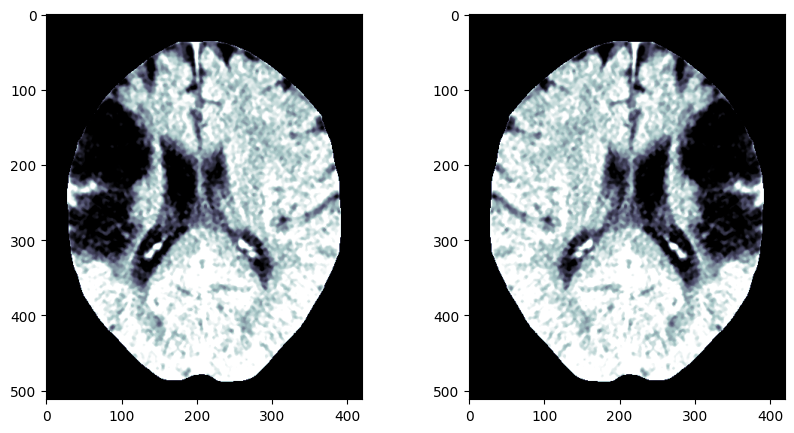
\includegraphics[width=\textwidth, keepaspectratio]{horizontal-flip.png}
% \caption[]{داده‌افزایی به روش قرینه‌سازی تصادفی افقی.}
% \label{fig:horizontal-flip}
% \end{figure}

\شروع{شکل}[ht]
\centerimg{horizontal-flip}{0.7\textwidth}
\شرح[داده‌افزایی به روش قرینه‌سازی تصادفی افقی]{داده‌افزایی به روش قرینه‌سازی تصادفی افقی}
\برچسب{fig:horizontal-flip}
\پایان{شکل}

روش دیگری که برای افزایش داده‌ها به‌کار گرفته‌شد، دوران مغز است. در این 
تغییر، محور عمودی مغز بین $-30$ تا $30$ درجه به صورت تصادفی دوران می‌یابد.
نمونه‌ی این تغییر در تصویر \ref{fig:rotation}
قابل مشاهده است.

% \begin{figure}[ht]
% \centering
% 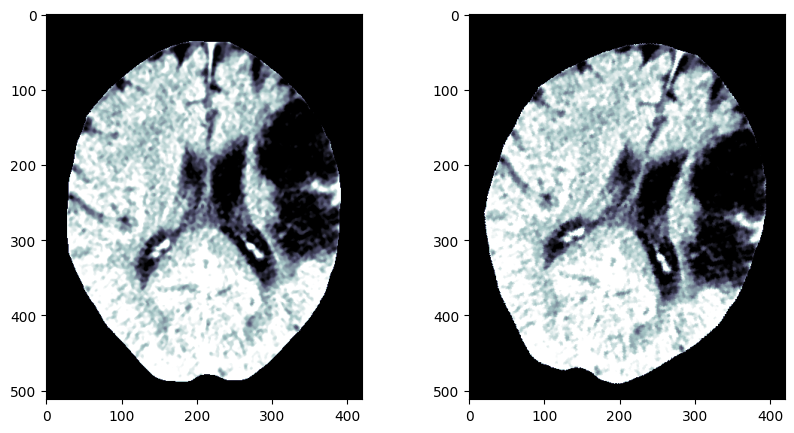
\includegraphics[width=\textwidth, keepaspectratio]{rotation.png}
% \caption[]{داده‌افزایی به روش دوران تصادفی.}
% \label{fig:rotation}
% \end{figure}

\شروع{شکل}[ht]
\centerimg{rotation}{0.7\textwidth}
\شرح[داده‌افزایی به روش دوران تصادفی]{داده‌افزایی به روش دوران تصادفی}
\برچسب{fig:rotation}
\پایان{شکل}

تکنیک دیگری که برای داده افزایی مورد استفاده قرار گرفته‌است،
جابجایی جزئی مغز در تصاویر است.
این جابجایی در حدود یک‌صدم اندازه‌ی تصویر صورت می‌گیرد.
نمونه‌ی این تغییر در تصویر 
\ref{fig:translate}
قابل مشاهده است.

% \begin{figure}[ht]
% \centering
% 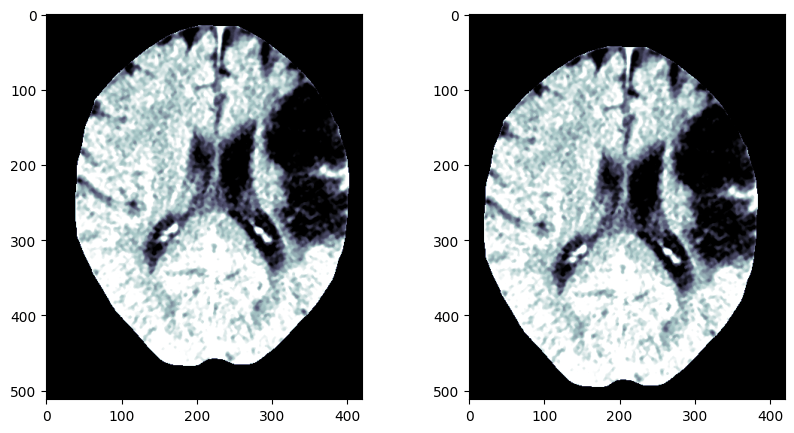
\includegraphics[width=\textwidth, keepaspectratio]{translate.png}
% \caption[]{داده‌افزایی به روش جابجایی تصادفی.}
% \label{fig:translate}
% \end{figure}

\شروع{شکل}[ht]
\centerimg{translate}{0.7\textwidth}
\شرح[داده‌افزایی به روش جابجایی تصادفی]{داده‌افزایی به روش جابجایی تصادفی}
\برچسب{fig:translate}
\پایان{شکل}

% \begin{figure}[ht]
% \centering
% 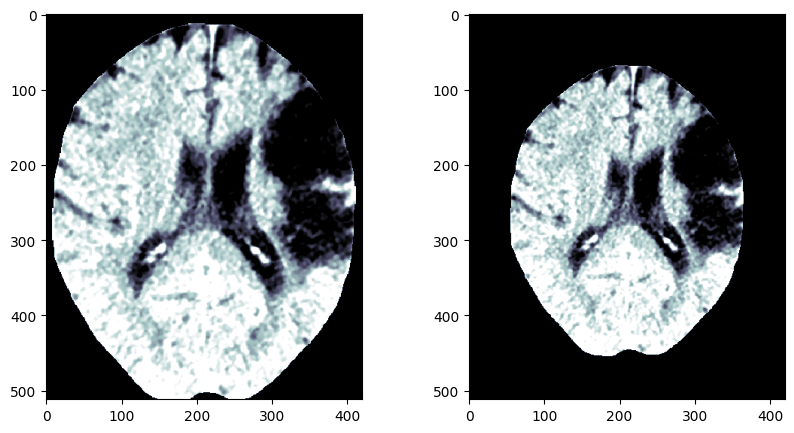
\includegraphics[width=\textwidth, keepaspectratio]{scale.png}
% \caption[]{داده‌افزایی به روش تغییر مقیاس تصادفی.}
% \label{fig:scale}
% \end{figure}

تغییر مقیاس تصادفی روش دیگری برای داده‌افزایی است که در این پروژه مورد استفاده قرار گرفته‌است.
افزایش و کاهش مقیاس تصاویر مغزی در حدود یک‌دهم اندازه‌ی اصلی تصویر صورت می‌گیرد.
یک نمونه از تبدیل مقیاس تصادفی در تصویر 
\ref{fig:scale} قابل مشاهده است.

\شروع{شکل}[ht]
\centerimg{scale}{0.7\textwidth}
\شرح[داده‌افزایی به روش تغییر مقیاس تصادفی]{داده‌افزایی به روش تغییر مقیاس تصادفی}
\برچسب{fig:scale}
\پایان{شکل}

دو روش دیگر برای افزایش داده‌ها،
 تبدیل برشی\footnote{Shearing}
تصادفی و 
زاویه‌ی دید\footnote{Perspective}
تصادفی هستند.
در یک تعریف غیر رسمی، تبدیل اول، تصویر مغز را کمی در راستای افقی کج‌تر می‌کند و تبدیل دوم، زاویه‌ی نگاه متفاوت به مغز را شبیه‌سازی می‌کند.
طبق آزمایش‌های انجام‌شده، تبدیل دوم برای افزایش داده‌ها تاثیر مطلوبی بر روی عملکرد مدل نداشته و در این پروژه به‌کار نیامده‌است.
نمونه‌ی این دو تبدیل به ترتیب در تصاویر \ref{fig:shear} و \ref{fig:perspective} آمده‌است.

% \begin{figure}[ht]
% \centering
% 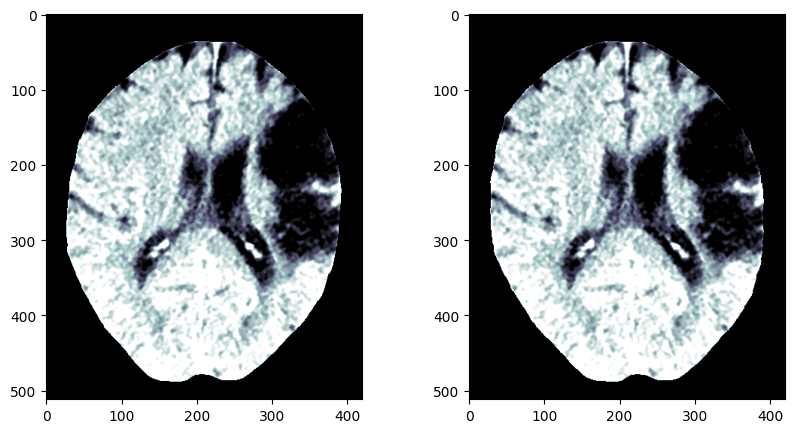
\includegraphics[width=\textwidth, keepaspectratio]{shear.png}
% \caption[]{داده‌افزایی به روش تبدیل برشی تصادفی.}
% \label{fig:shear}
% \end{figure}

\شروع{شکل}[ht]
\centerimg{shear}{0.7\textwidth}
\شرح[داده‌افزایی به روش تبدیل برشی تصادفی]{داده‌افزایی به روش تبدیل برشی تصادفی}
\برچسب{fig:shear}
\پایان{شکل}


% \begin{figure}[ht]
% \centering
% 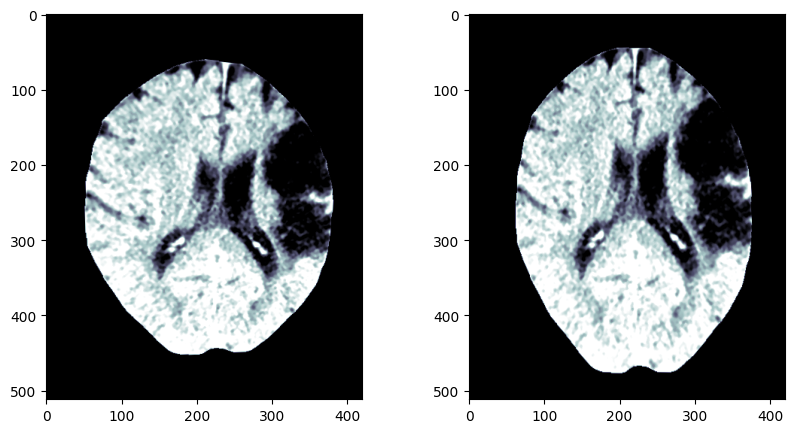
\includegraphics[width=\textwidth, keepaspectratio]{perspective.png}
% \caption[]{داده‌افزایی به روش زاویه‌ی دید تصادفی.}
% \label{fig:perspective}
% \end{figure}

\شروع{شکل}[ht]
\centerimg{perspective}{0.7\textwidth}
\شرح[داده‌افزایی به روش زاویه‌ی دید تصادفی]{داده‌افزایی به روش زاویه‌ی دید تصادفی}
\برچسب{fig:perspective}
\پایان{شکل}

آخرین تکنیکی که برای افزایش داده‌ها قابل استفاده می‌باشد،، 
مات‌سازی گاوسی\footnote{\lr{Gaussian Blur}}
تصادفی است.
در این روش، مقدار هر پیکسل با میانگین وزن‌داری از یک همسایگی آن پیکسل جایگزین می‌شود.
به این ترتیب، تصویر قدری محو‌تر و درهم‌تنیده‌تر دیده‌می‌شود.
این تبدیل نیز طی آزمایش‌های صورت‌گرفته، در بهبود عملکرد مدل تاثیر مطلوبی نداشته و در این پژوهش مورد استفاده قرار نگرفته‌است.
شکل \ref{fig:gaussian} یک نمونه از این نوع داده‌افزایی را نشان می‌دهد.
البته در این تصویر، به منظور نمایش بهتر، اندازه‌ی فیلتر گاوسی مقدار بزرگی در نظر گرفته شده.

% \begin{figure}[ht]
% \centering
% 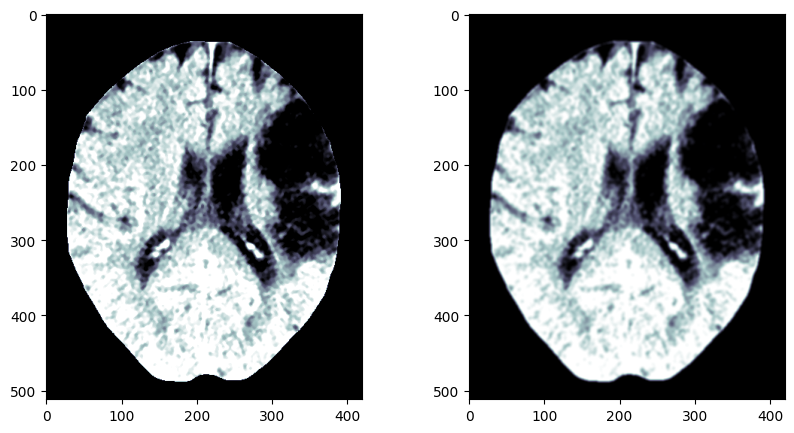
\includegraphics[width=\textwidth, keepaspectratio]{gaussian.png}
% \caption[]{داده‌افزایی به روش مات‌سازی گاوسی تصادفی.}
% \label{fig:gaussian}
% \end{figure}

\شروع{شکل}[ht]
\centerimg{gaussian}{0.7\textwidth}
\شرح[داده‌افزایی به روش مات‌سازی گاوسی تصادفی]{داده‌افزایی به روش مات‌سازی گاوسی تصادفی}
\برچسب{fig:gaussian}
\پایان{شکل}

تمام تکنیک‌های مذکور به صورت تصادفی بر روی هر تصویر پیش‌پردازش‌شده اعمال شده و نتیجه‌ی آن‌ها
به مدل ورودی داده می‌شوند.
به این ترتیب، مجموعه‌داده‌ی در دسترس، با تغییراتی جزئی، افزایش حجم قابل توجهی می‌یابد.
باید توجه داشت که این تغییرات، شکل آسیب‌دیدگی را تغییر نمی‌دهند و تنوع موارد سکته‌ی مغزی‌ای که مدل می‌بیند را 
افزایش نمی‌دهند.
بلکه تنها باعث می‌شوند نمونه‌های موجود به صورت مطمئن‌تری فراگرفته شوند.
درواقع تنوع به‌وجود آمده، باعث می‌شود مدل، ظاهر خاص داده‌های ورودی را حفظ نکند. بلکه ویژگی‌های کلیدی آن‌ها را فرابگیرد.

\قسمت{ساختار ورودی و خروجی}

همانطور که پیش‌تر ذکر شد، به ازای هر بیمار تعداد زیادی تصویر از برش‌های مختلف مغز وی وجود دارد.
پژوهش‌ها‌ی مختلف بر روی تعداد متفاوتی از این تصاویر کار می‌کنند.
برخی از آن‌ها تمام برش‌ها را مورد بررسی قرار داده و یک مطالعه‌ی سه‌بعدی انجام می‌دهند.
برخی نیز بر روی تنها دو برش خاص از مغز کار می‌کنند.
در این قسمت ابتدا ساختار ورودی مدل ارائه‌شده در این پروژه ذکر می‌شود
و مشخص می‌شود که
این ساختار، حالت میانه‌ای از دو حالت ذکر شده می‌باشد.

در مورد فرمت خروجی مدل پژوهش‌های مشابه نیز با هم تفاوت‌هایی وجود دارد.
برخی از کارهای پیشین با دریافت تصاویر یک بیمار، یک امتیاز از صفر تا ۱۰ خروجی می‌دهند و برخی، امتیاز ASPECTS را به صورت دوبخشی محاسبه می‌کنند.
یعنی بالاتر و پایین‌تر بودن امتیاز ASPECTS نسبت به یک عدد آستانه را مشخص می‌کنند.
در ادامه، فرمت خروجی مدل پیشنهادی نیز شرح داده‌می‌شود و
مجددا مشاهده می‌شود که این ساختار، حالت میانه‌ای از دو نوع ذکرشده است که برخواسته از محدودیت‌های داده‌ای می‌باشد.

\زیرقسمت{ساختار ورودی}

تصویر \ref{fig:aspects-regions}
در فصل مفاهیم اولیه، دو برش به‌خصوص از مغز را نشان می‌دهد که بخش‌هایی از هر ۱۰ ناحیه‌ی ASPECTS را در برمی‌گیرند.
اما حجم واقعی این نواحی، به همین دو برش محدود نمی‌شود.
بلکه در چندین برش از مغز گسترده شده‌است.
شکل \ref{fig:aspects-slices}
از همین بخش، ۸ برش مغز را نشان می‌دهد که تقریب بهتری از این نواحی هستند و گستردگی آن‌ها را تا حد بسیار خوبی پوشش می‌دهند.
در عمل نیز متخصصان
ناحیه‌های ASPECTS را 
 نه فقط در دو برش خاص از مغز، بلکه 
 در چندین برش مجاور منطبق بر کالبدشناسی تصویر 
 \ref{fig:aspects-slices}
 مشاهده می‌کنند.

 بنابراین به نظر می‌رسد که بررسی این ۸ برش، به واقعیت تشخیص‌های انسانی نزدیک‌تر است.
 یکی از نقاط قوت این پژوهش نیز از همین موضوع نشأت می‌گیرد.
 در این پروژه، ۶ برش از مغز بیماران، به مدل ورودی داده‌می‌شود.
این در حالی است که در جستجویی که در کارهای پیشین
انجام شد، این کارها یا ورودی کاملاً سه‌بعدی داشتند و تمام برش‌ها را بررسی می‌کردند و یا تنها دو برش خاص از مغز را به مدل ورودی می‌دادند.

بررسی تنها دو برش از تصاویر ورودی می‌تواند قابلیت اطمینان تشخیص مدل را کاهش دهد.
چرا که قسمت اعظم برخی آسیب‌دیدگی‌های مشاهده‌شده
بر روی برش‌های فوقانی یا تحتانی مغز می‌باشد که از دید این مدل‌ها پنهان می‌ماند.
بنابراین امید می‌رود که روش انتخابی در این پروژه که انطباق بیشتری با واقعیت دارد، عملکرد بهتری از خود نشان بدهد.

همانطور که گفته شد، مدل پیشنهادی، ۶ برش مغزی از هر بیمار را ورودی می‌گیرد.
 برش‌های انتخابی در تصویر \ref{fig:aspects-selected-slices} مشخص شده‌اند.
 عدم استفاده از برش‌های اول و هشتم 
به دو دلیل صورت گرفته‌است.
اول آنکه این برش‌ها، نسبت به سایر برش‌های میانی اطلاعات کمتری دارند و حذف آن‌ها می‌تواند فرایند یادگیری را برای مدل ساده‌تر کند.
به طور دقیق‌تر، کاهش تعداد ویژگی‌های ورودی، می‌تواند از 
بیش‌برازش\footnote{Overfitting}
مدل جلوگیری کند.
دوم آنکه برش اول در بسیاری از بیماران، در سطحی از مغز اتخاذ شده‌بود که 
بخشی از بافت استخوانی در بافت مغزی نفوذ کرده‌بود.
این مسئله سبب چند‌بخشی‌شدن مغز و ایجاد تنوع زیادی در بافت استخراج‌شده‌ی مغزی می‌شد و یادگیری را برای مدل مشکل می‌کرد.

\شروع{شکل}[ht]
\centerimg{aspects-selected-slices}{\textwidth}
\شرح[برش‌های انتخابی ASPECTS]{برش‌های انتخابی ASPECTS}
\برچسب{fig:aspects-selected-slices}
\پایان{شکل}

\زیرقسمت{ساختار خروجی}

خروجی نهایی مدل پروژه از تصاویر هر بیمار، امتیاز دوبخشی ASPECTS است.
به طور دقیق‌تر، مدل تشخیص می‌دهد که ASPECTS بیمار $\geq 6$ است یا $<6$.
اما در صورتی که مدل با همین خروجی آموزش داده‌شود،
نمی‌تواند به خوبی فرابگیرد.
چرا که در این حالت،
مجموعه‌ی بسیار متنوعی از تصاویر مغزی از
امتیاز ۶ گرفته تا ۱۰، همگی با برچسب
$\geq6$ به مدل عرضه می‌شوند.
پیدا کردن یک الگوی مشترک میان این مجموعه‌ی متنوع، برای مدل دشوار است.
اما در صورتی که به مدل یک راهنمایی صورت بگیرد که دقیقاً مشخص می‌کند هر تصویر متعلق به کدام امتیاز از ۶ تا ۱۰ است، مدل می‌تواند میان تصاویر مربوط به هر امتیاز، الگوی مشترکی پیدا کرده و آن امتیاز را فرابگیرد.

درواقع بهتر آن است که حقایق و اطلاعات پزشکی بیشتری برای مدل فراهم شود و آموزشش در حالت ۱۰ امتیازی ASPECTS انجام شود.
اما همانطور که در فصل کار‌های پیشین مشاهده شد، برای هر یک از امتیاز‌های $<6$، تعداد بسیار اندکی تصویر وجود دارد.
به نحوی که در مجموع تنها ۱۱ بیمار با این امتیازات وجود دارد.
بنابراین مدل نمی‌تواند با این تعداد نمونه‌ی اندک، دسته و مجموعه‌ای برای آن امتیاز را آموزش ببیند.
به علت همین محدودیت، در این پروژه، حالت میانه‌ای از آموزش دو-کلاسه و ۱۱-کلاسه در پیش گرفته‌شده‌است.
به نحوی که مدل بر روی 6 دسته‌ی $0-5$، 6، 7، 8، 9 و 10 آموزش می‌بیند و خروجی نهایی آن،‌ دوبخشی شده و گزارش می‌شود.

\قسمت{طراحی مدل}

پس از پیش‌پردازش داده‌ها و بررسی ساختار ورودی و خروجی مدل، نوبت به هسته‌ی مرکزی مدل، یعنی ساختار شبکه‌ی آن می‌رسد.
همانطور که در فصل مفاهیم اولیه آمد، یکی از راه‌های مدیریت حجم محدود داده‌ها، روش یادگیری انتقالی است.
در این پروژه نیز، از این روش استفاده می‌شود و یک مدل پیش‌آموزش‌دیده، به عنوان پایه‌ی شبکه‌ی پیشنهادی قرار می‌گیرد.
پس از بررسی مدل‌های پیش‌آموزش‌دیده‌ی مختلف، از جمله مدل‌های ،DenseNet ،ResNet \lr{InceptionV3}، ،SqueezeNet ،AlexNet VGG و \lr{EfficientNetV2}، مشخص شد که مدل \lr{EfficientNetB0} بهتر از همه نتیجه می‌دهد و لذا 
در این پروژه به‌کار گرفته‌شده‌است.

مدل \lr{EfficientNetB0} میلیون‌ها پارامتر دارد و بر روی میلیون‌ها تصویر آموزش دیده‌است تا آن‌ها را در ۱۰۰۰ دسته طبقه‌بندی کند.
تصاویر ورودی و دسته‌های خروجی در مدل مورد نیاز ما متفاوت هستند. اما
همان‌گونه که پیش‌تر گفته شد، به کمک یادگیری انتقالی می‌توان از توانایی مدل \lr{EfficientNetB0} برای تشخیص اشکال مختلف و استخراج ویژگی‌های آن‌ها بهره برد.

مدل \lr{EfficientNetB0} یک تصویر دو‌بعدی رنگی را ورودی می‌گیرد، یک‌سری ویژگی‌های کلیدی آن را استخراج می‌کند و 
سپس در چند لایه‌ی انتهایی مدل، که به آن قسمت 
طبقه‌بندی‌کننده\footnote{Classifier}
گفته می‌شود، تصویر را در یکی از دسته‌های خروجی خود قرار می‌دهد.
در یادگیری انتقالی، قسمت طبقه‌بندی‌کننده از مدل پیش‌آموزش‌دیده حذف می‌شود.
به این ترتیب تنها از قسمتی از مدل استفاده می‌شود که ویژگی‌ها را از تصاویر استخراج می‌کنند.

همانطور که گفته‌شد، مدل \lr{EfficientNetB0} تنها یک تصویر را دریافت و پردازش می‌کند.
از آن‌جا که مدل پیشنهادی در این پروژه، ۶ تصویر ورودی دارد، برای استخراج ویژگی‌های این تصاویر، ۶ 
نمونه\footnote{Instance}
از مدل \lr{EfficientNetB0} گرفته می‌شود.
ویژگی‌های استخراج شده از هر تصویر، پشت یک لایه‌ی 
جدید قرار می‌گیرند تا یک مرحله پردازش شده و به منظور خاص پروژه نزدیک‌تر شوند.
سپس این ویژگی‌های خاص‌منظوره‌تر، همگی با هم الصاق می‌شوند و طی دو لایه‌ی جدید دیگر، طبقه‌بندی نهایی تصاویر را انجام می‌دهند.
با این توضیحات، ساختار نهایی شبکه در تصویر \ref{fig:network}
قابل مشاهده است.
جزئیات این شبکه، 
طی آزمایش تعداد بسیار زیادی ساختار مختلف و ارزیابی نتایج حاصل از آن‌ها به صورت تجربی به‌دست آمده‌است.

% \begin{figure}[ht]
% \centering
% 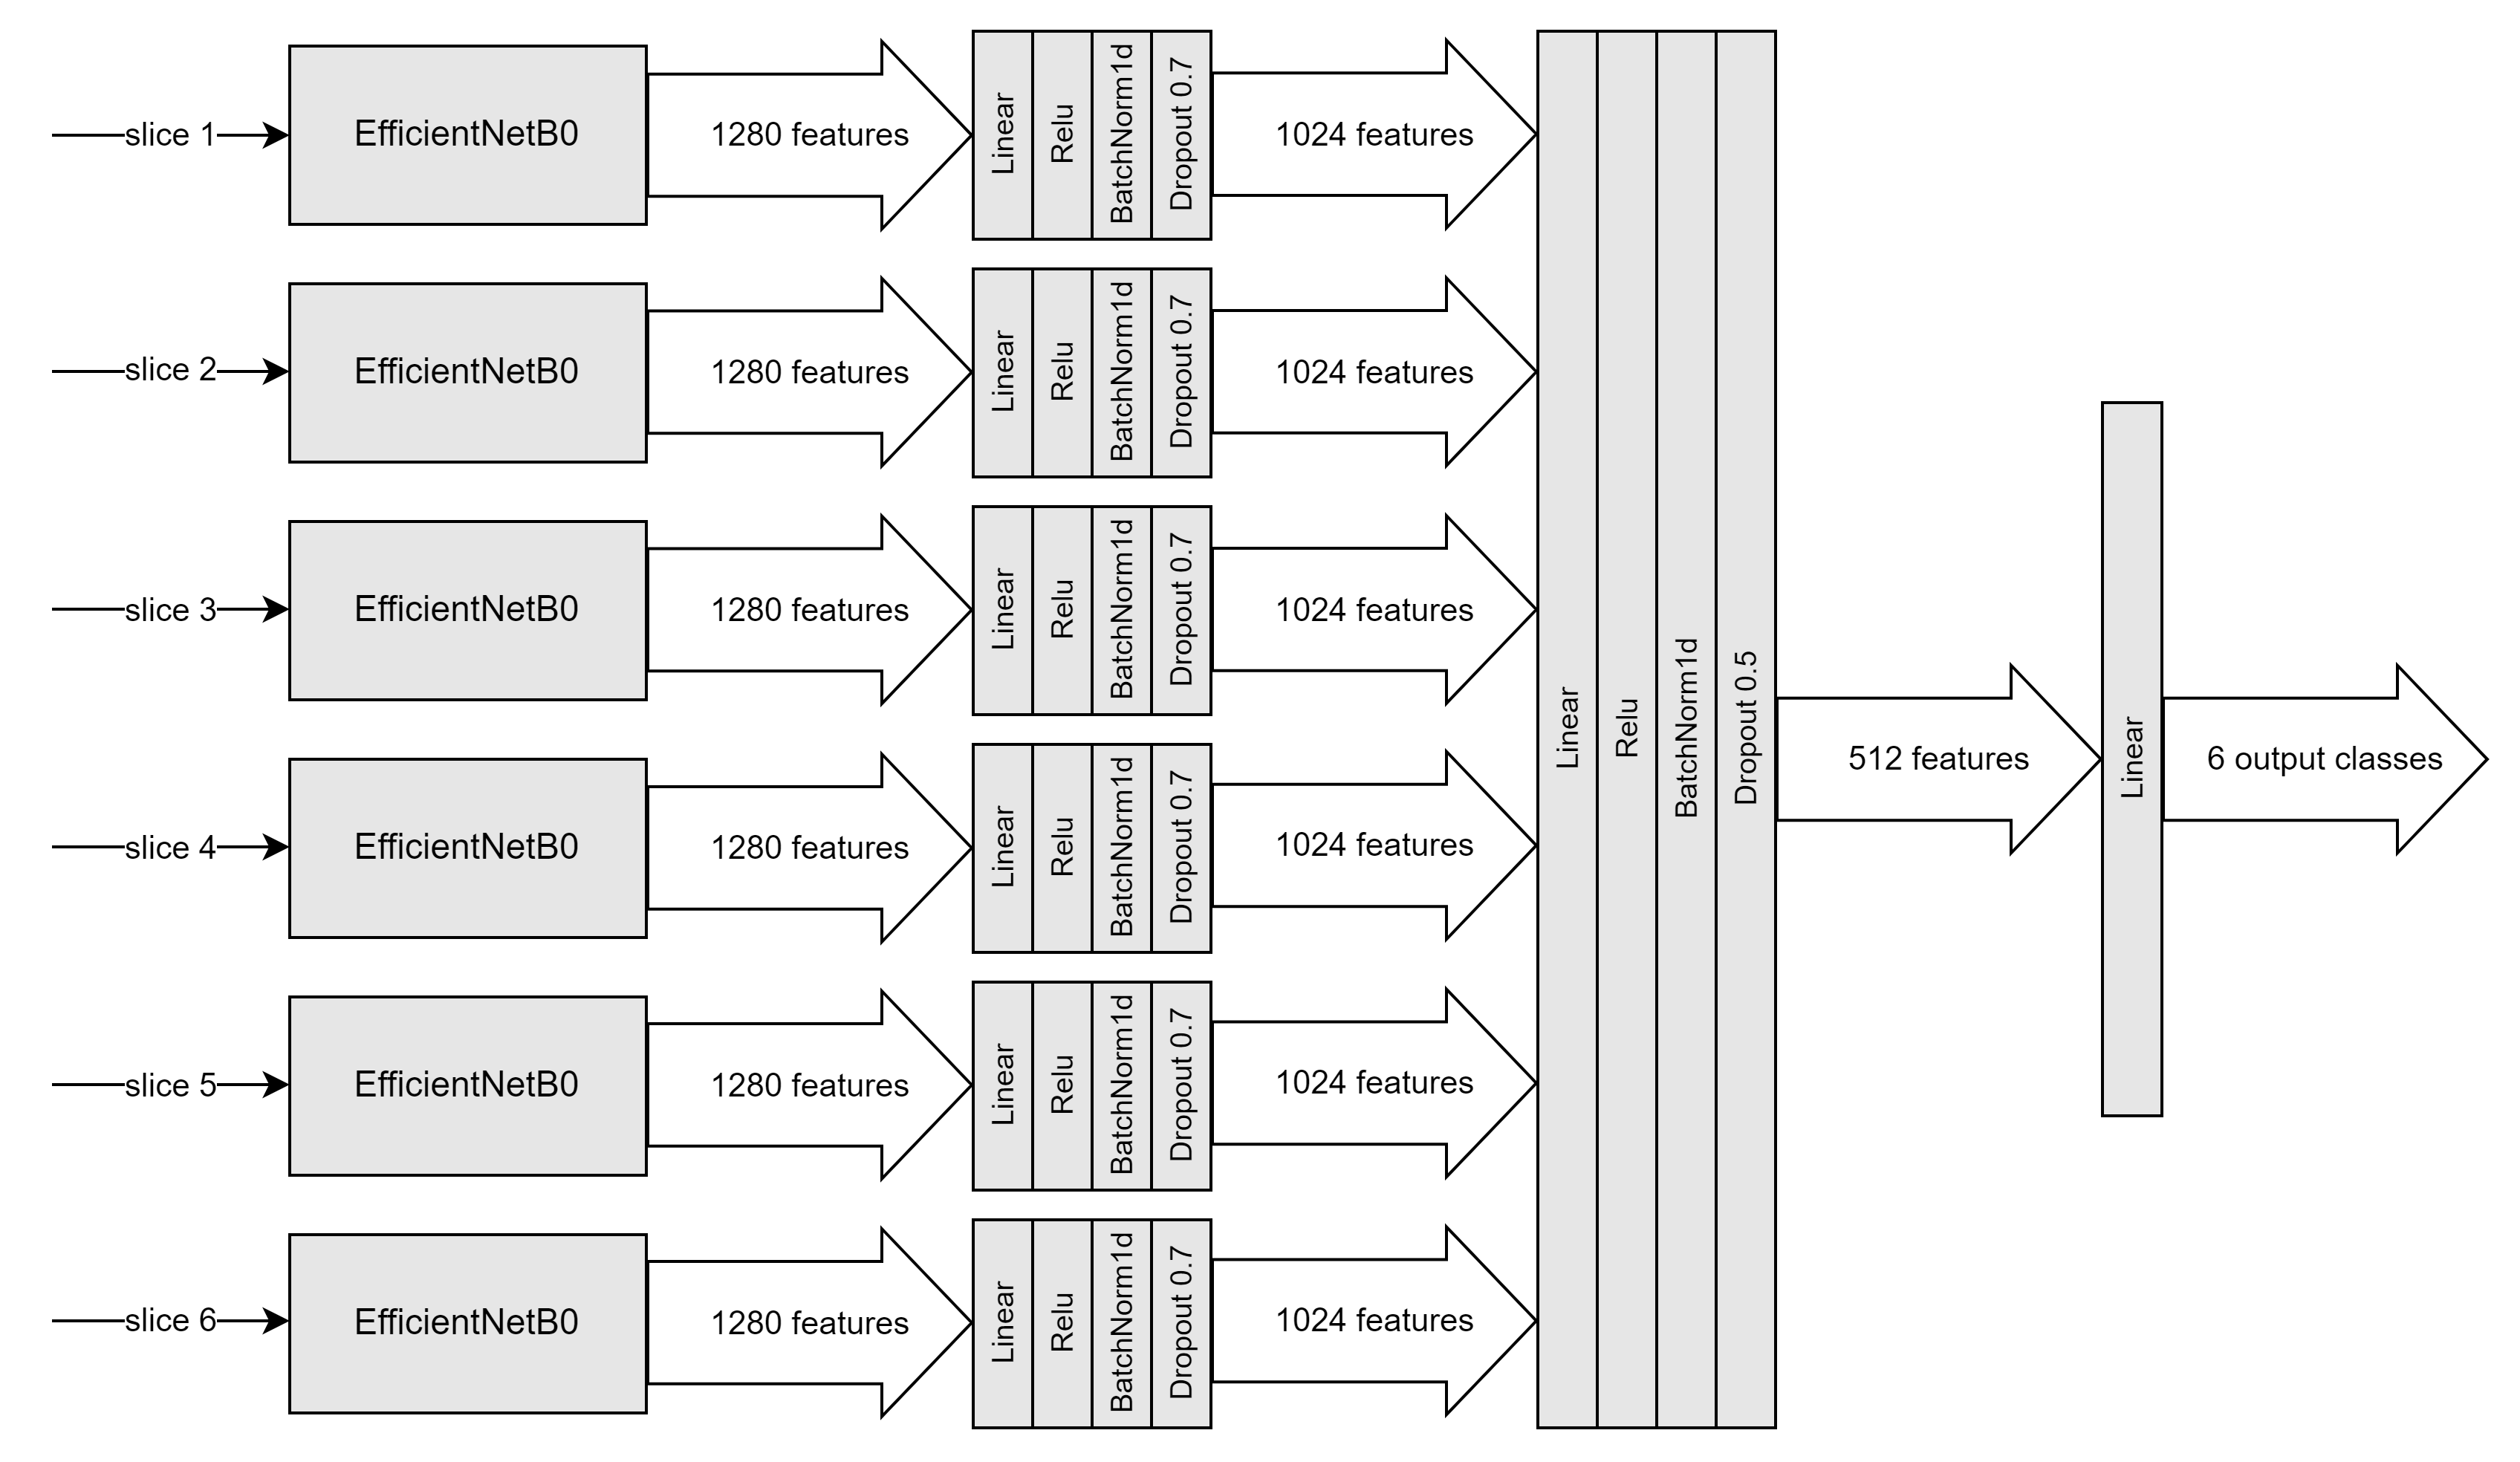
\includegraphics[width=\textwidth, keepaspectratio]{network.png}
% \caption[]{ساختار نهایی شبکه.}
% \label{fig:network}
% \end{figure}

\شروع{شکل}[ht]
\centerimg{network}{\textwidth}
\شرح[ساختار شبکه‌ی پیشنهادی]{ساختار شبکه‌ی پیشنهادی}
\برچسب{fig:network}
\پایان{شکل}


\قسمت{جمع‌بندی}

در این فصل به شرح هسته‌ی اصلی پژوهش، یعنی روش حل مسئله، پرداخته‌شد.
ترتیب فعالیت‌های انجام‌شده برای حل مسئله در این پروژه، منطبق بر عناوین همین فصل بوده‌است.
درواقع در ابتدا، اطلاعات دریافتی از مرکز درمانی مربوطه، گرد‌آوری و مرتب شده‌اند.
سپس چهارچوب ورودی مدل، با توجه به مفاهیم پزشکی و روش‌های مورد استفاده توسط متخصصان تعیین گشته‌است.
همچنین با توجه به نیازمندی‌های پروژه و تا حدی محدودیت‌های حاکم بر آن، قالب خروجی مدل به صورت دوبخشی انتخاب شده‌است.
در ادامه نیز
طراحی مدل انجام شده و طی آزمایش‌های بسیار، دچار تغییر و تحول گشته تا به حالت نهایی خود به صورتی که در این فصل ذکر شد، رسیده‌است.
فصل‌های بعدی پایان‌نامه به ارزیابی و تحلیل جایگاه این روش اختصاص خواهد داشت.